\section{Chapter 12}
\subsection{12.1}
\begin{itemize}
    \item[2.] Find the values, if any, of the Boolean variable x that
          satisfy these equations.
          \begin{tasks}(4)
              \task $x \cdot 1 = 0$
              \task $x + x = 0$
              \task $x \cdot 1 = x$
              \task $x \cdot \overline{x} = 1$
          \end{tasks}
          \answer
          \begin{tasks}(4)
              \task $x = 0$
              \task $x = 0$
              \task $x = 1,\ x = 0$
              \task No value of x satisfies.
          \end{tasks}

    \item[6.]  Use a table to express the values of each of these Boolean
          functions.
          \begin{tasks}(2)
              \task $F(x, y, z) = \overline{z}$
              \task $F(x, y, z) = \overline{x}y + \overline{y}z$
              \task $F(x, y, z) = x\overline{y}z + \overline{(xyz)}$
              \task $F(x, y, z) = \overline{y}(xz + \overline{x}\, \overline{z})$
          \end{tasks}

          \answer

          \begin{tasks}(2)
              \task \text{}\\
              \begin{tabular}{*{4}{|c}|}
                  $x$ & $y$ & $z$ & $\overline{z}$ \\
                  \hline
                  1   & 1   & 1   & 0              \\
                  1   & 1   & 0   & 1              \\
                  1   & 0   & 1   & 0              \\
                  1   & 0   & 0   & 1              \\
                  0   & 1   & 1   & 0              \\
                  0   & 1   & 0   & 1              \\
                  0   & 0   & 1   & 0              \\
                  0   & 0   & 0   & 1              \\
                  \hline
              \end{tabular}

              \task \text{}\\
              \begin{tabular}{*{6}{|c}|}
                  $x$ & $y$ & $z$ & $\overline{x}y$ & $x\overline{y}$ & $\overline{x}y + \overline{y}z$ \\
                  \hline
                  1   & 1   & 1   & 0               & 0               & 0                               \\
                  1   & 1   & 0   & 0               & 0               & 0                               \\
                  1   & 0   & 1   & 0               & 1               & 1                               \\
                  1   & 0   & 0   & 0               & 0               & 0                               \\
                  0   & 1   & 1   & 1               & 0               & 1                               \\
                  0   & 1   & 0   & 1               & 0               & 1                               \\
                  0   & 0   & 1   & 0               & 1               & 1                               \\
                  0   & 0   & 0   & 0               & 0               & 0                               \\
                  \hline
              \end{tabular}

              \task \text{}\\
              \begin{tabular}{*{6}{|c}|}
                  $x$ & $y$ & $z$ & $x\overline{y}z$ & $\overline{(xyz)}$ & $x\overline{y}z + \overline{(xyz)}$ \\
                  \hline
                  1   & 1   & 1   & 0                & 0                  & 0                                   \\
                  1   & 1   & 0   & 0                & 1                  & 1                                   \\
                  1   & 0   & 1   & 1                & 1                  & 1                                   \\
                  1   & 0   & 0   & 0                & 1                  & 1                                   \\
                  0   & 1   & 1   & 0                & 1                  & 1                                   \\
                  0   & 1   & 0   & 0                & 1                  & 1                                   \\
                  0   & 0   & 1   & 0                & 1                  & 1                                   \\
                  0   & 0   & 0   & 0                & 1                  & 1                                   \\
                  \hline
              \end{tabular}

              \task \text{}\\
              \begin{tabular}{*{6}{|c}|}
                  $x$ & $y$ & $z$ & $xz$ & $\overline{x}\, \overline{z}$ & $\overline{y}(xz + \overline{x}\, \overline{z})$ \\
                  \hline
                  1   & 1   & 1   & 1    & 0                             & 0                                                \\
                  1   & 1   & 0   & 0    & 0                             & 0                                                \\
                  1   & 0   & 1   & 1    & 0                             & 1                                                \\
                  1   & 0   & 0   & 0    & 0                             & 0                                                \\
                  0   & 1   & 1   & 0    & 0                             & 0                                                \\
                  0   & 1   & 0   & 0    & 0                             & 0                                                \\
                  0   & 0   & 1   & 0    & 0                             & 0                                                \\
                  0   & 0   & 0   & 0    & 1                             & 1                                                \\
                  \hline
              \end{tabular}
          \end{tasks}

    \item[10.]  How many different Boolean functions are there of degree 7?\\
          \answer \\
          $2^{2^7} = 2^{128}$

    \item[12.]  Show that $F (x, y, z) = xy + xz + yz$ has the value 1 if
          and only if at least two of the variables $x,\ y,\ \text{and } z$ have
          the value 1. \\
          \answer \\
          The function has all the possible 2 combinations of $x,y,z$ as products being summed together.
          The only way one of those products has the value of one is if both variables are 1. So
          at least 2 of $x,y,\ \text{and } z$ must be 1.

    \item[24.]  Simplify these expressions.
          \begin{tasks}(2)
              \task $x \oplus 0$
              \task $x \oplus 1$
              \task $x \oplus x$
              \task $x \oplus \overline{x}$
          \end{tasks}
          \answer
          \begin{tasks}(2)
              \task $x$
              \task $\overline{x}$
              \task 0
              \task 1
          \end{tasks}

    \item[28.]  Find the duals of these Boolean expressions.
          \begin{tasks}(2)
              \task $x + y$
              \task $\overline{x}\, \overline{y}$
              \task $xyz + \overline{x}\, \overline{y}\, \overline{z}$
              \task $x\overline{z} + x \cdot 0 + \overline{x} \cdot 1$
          \end{tasks}
          \answer
          \begin{tasks}(2)
              \task $xy$
              \task $\overline{x} + \overline{y}$
              \task $(x + y + z)(\overline{x} + \overline{y} + \overline{z})$
              \task $(x+\overline{z})(x+0)(\overline{x}+1)$
          \end{tasks}



\end{itemize}

\subsection{12.2}
\begin{itemize}
    \item[2.]  Find the sum-of-products expansions of these Boolean
          functions.
          \begin{tasks}(2)
              \task $F (x, y) = \overline{x} + y$
              \task $F (x, y) = x\, \overline{y}$
              \task $F (x, y) = 1$
              \task $F (x, y) = \overline{y}$
          \end{tasks}
          \answer
          \begin{tasks}(2)
              \task $xy + \overline{x} y + \overline{x}\,\overline{y}$
              \task $x\overline{y}$
              \task $xy + \overline{x} y + x\overline{y}+\overline{x}\,\overline{y}$
              \task $x\overline{y} + \overline{x}\,\overline{y}$
          \end{tasks}

    \item[4.] Find the sum-of-products expansions of the Boolean
          function $F (x, y, z)$ that equals 1 if and only if
          \begin{tasks}(2)
              \task $x = 0.$
              \task $xy = 0.$
              \task $x + y = 0.$
              \task $xyz = 0.$
          \end{tasks}
          \answer
          \begin{tasks}(2)
              \task $\overline{x}yz + \overline{x}\,\overline{y}z + \overline{x}y\overline{z} + \overline{x}\,\overline{y}\,\overline{z}$
              \task $\overline{x}yz + \overline{x}\,\overline{y}z + \overline{x}y\overline{z} + \overline{x}\,\overline{y}\,\overline{z} + x\overline{y}z + x\overline{y}\,\overline{z}$
              \task $\overline{x}\,\overline{y}z + \overline{x}\,\overline{y}\,\overline{z}$
              \task $\overline{x}yz + \overline{x}\,\overline{y}z + \overline{x}y\overline{z} + \overline{x}\,\overline{y}\,\overline{z} + x\overline{y}z + x\overline{y}\,\overline{z} + xy\overline{z}$
          \end{tasks}

    \item[6.]  x, y,  z  Find the sum-of-products expansion of the
          Boolean function $F(x_1 , x_2 , x_3 , x_4, x_5)$ that has the value 1
          if and only if three or more of the variables
          $x_1 , x_2 , x_3, x_4$, and $x_5$ have the value 1. \\
          \answer \\
          $x_1 x_2 x_3 x_4 x_5 + \overline{x_1} x_2 x_3 x_4 x_5 + x_1 \overline{x_2} x_3 x_4 x_5 + x_1 x_2 \overline{x_3} x_4 x_5 + x_1 x_2 x_3 \overline{x_4} x_5 + x_1 x_2 x_3 x_4 \overline{x_5} + \overline{x_1}\,\overline{x_2} x_3x_4 x_5 + x_1 \overline{x_2}\,\overline{x_3} x_4 x_5 + x_1 x_2\overline{x_3}\,\overline{x_4}x_5 + x_1 x_2 x_3 \overline{x_4}\,\overline{x_5} + \overline{x_1}x_2 \overline{x_3}x_4 x_5 + \overline{x_1}x_2 x_3 \overline{x_4} x_5  + \overline{x_1}x_2x_3x_4\overline{x_5} + x_1\overline{x_2}x_3\overline{x_4}x_5 + x_1\overline{x_2}x_3x_4\overline{x_5} + x_1x_2\overline{x_3}x_4\overline{x_5}$


\end{itemize}

\subsection{12.3}
For exercises 2 and 4 find the output of the given circuit.
\begin{itemize}
    \item[2.] \text{} \\
          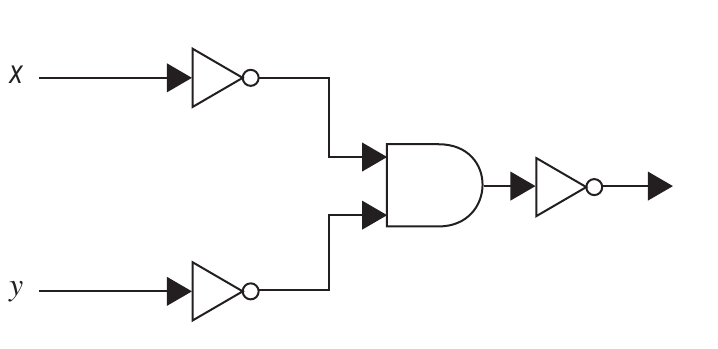
\includegraphics[scale = 0.6]{img/12_3_2_circuit.png} \\
          \answer \vspace{1mm}\\
          $\overline{\overline{x}\,\overline{y}}$

    \item[4.] \text{} \\
          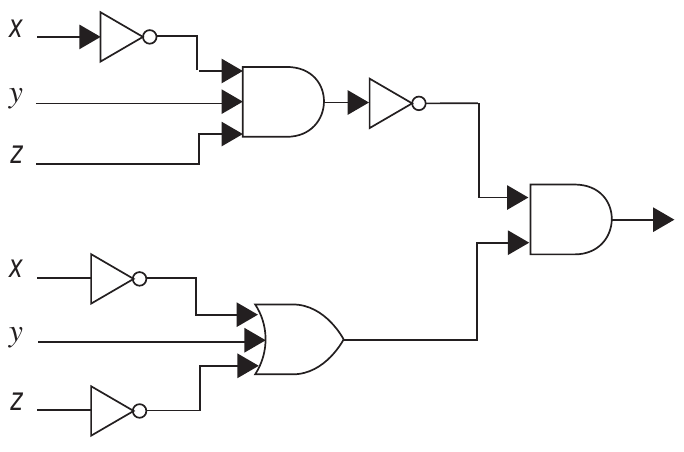
\includegraphics[scale = 0.6]{img/12_3_4_circuit.png} \\
          \answer \vspace{1mm}\\
          $\overline{(\overline{x}yz)}(\overline{x} + y + \overline{z})$

    \item[6.]  Use NOR gates to construct circuits for the outputs given
    \begin{tasks}(3)
          \task $\overline{x}$
          \task $x + y$
          \task $xy$
    \end{tasks}
    \answer
    \begin{tasks}(3)
        \task $x \downarrow x$
        \task $(x \downarrow y) \downarrow (x \downarrow y)$
        \task $(x \downarrow x) \downarrow (y \downarrow y)$
    \end{tasks}

\end{itemize}